% $Id$

%\section{Motivation for Hardware Injections}
%\label{s:motivation}
Gravitational radiation incident on the LIGO interferometers from an
inspiralling binary will cause the test masses to move relative to each other.
This produces a differential change in length of the arms as described in
section \ref{s:effect}.  \emph{Injection} is the process of adding a waveform to
interferometer data to simulate the presence of a signal in the noise. We use
injections to measure the performance of the binary inspiral analysis
pipeline as described in section \ref{s:eff}.  \emph{Software injections},
which add a simulated signal to the data after it has been recorded, are used
for efficiency measurements. Since they performed \emph{a posteriori} the
interferometer is not affected while it is recording data.  Alternatively, a
simulated signal can be added to the interferometer control system to make the
instrument behave as if an inspiral signal is present.  The interferometer
Length Sensing and Control system has excitation points which allow arbitrary
signals to be added into the servo control loops or to the drives that control
the motion of the mirrors\cite{LIGOS1instpaper}.  We call this \emph{hardware
injection}; the data recorded from the instrument contains the simulated
signal. Figure \ref{f:ifo_inj} shows the hardware injection points on a
schematic diagram of the interferometer and length sensing and control loop.

Analysis of hardware injections allows us to ensure that the analysis pipeline
is sensitive to real inspiral signals and validates the software injections
used to test the pipeline efficiency.  In order to perform an accurate upper
limit analysis for binary inspirals, we must measure the efficiency of our
pipeline. That is, we inject a known number of signals into the pipeline and
determine the fraction of these detected.  Injecting signals into the
interferometer for the duration of a run is not practical and would
contaminate the data, so we use the analysis software to inject inspiral
signals into the data.  By comparing software and hardware injections we
confirm that software injections are adequate to measure the efficiency of the
upper limit pipeline.

Hardware injections provide a very complete method of testing the inspiral
detection pipeline. By recovering the physical parameters of an injected
signal, we test our understanding of all aspects of the pipeline, including
the instrumental calibration, the filtering algorithm and veto safety. We
injected inspiral signals immediately after the first LIGO science run (S1) in
September 2002. The resulting data was analyzed using the
software tools used to search for real signals.  In this chapter, we describe
the results of analysis of the S1 hardware injections. The analysis pipeline
used in S1 differs from that used in S2\cite{LIGOS1iul}. Here we are examining
the response of the filtering code to the hardware injections, however, and so
the differences between the S1 and S2 pipelines are unimportant.

\section{Injection of the Inspiral Signals}
\label{s:injecting}

To inject the signals, we generate the interferometer strain $h(t)$ produced
by an inspiralling binary using the restricted second order post-Newtonian
approximation in the time domain\cite{Blanchet:1996pi}.  The LSC calibration group
supplies a transfer function $T(f)$ which allows us to construct a signal
$g(t)$ that produces the desired strain when it is injected into the
interferometer.  The transfer function $T(f)$ should be identical to the
actuation function $A(f)$ described in section \ref{ss:calibration}, however
in S1 this was simplified to contain only the pendulum response of the mirrors,
given by 
\begin{equation}
T(f) = \frac{L}{C}\frac{f^2}{f_0^2}
\end{equation}
where $L$ is the length of the interferometer, $C$ is the calibration of the
excitation point in nm/count and $f_0$ is the pendulum frequency of the test
mass. Damping is neglected as it is unimportant in the LIGO frequency band.
The code used to generate the hardware injections is the same as that used
for software injections; only the transfer function used to generate the
injected signal differs since we are injecting into the control signal $g$
rather then the error signal $v$.

During S1, we injected signals corresponding to an optimally oriented binary.
Injections of two $1.4\,M_\odot$ neutron stars at distances from $10$ kpc to
$80$ kpc were used to test the neutron star analysis. 
We also injected signals from a $1.4,\,4.0\,M_\odot$ binary and several
$1.4,1.4\,M_\odot$ binaries at closer distances.  These signals were injected
into the differential mode servo and directly into an end test mass drive.

\section{Detection of the Injected Signals}
\label{s:detection}

Figure \ref{f:inj_snr} shows the events generated by processing 4000 seconds
of data from the Livingston 4 km interferometer (L1) on 10 September 2002
during the post-run hardware injections.

The first set of injections were large amplitude signals used to verify the
inspirals were being correctly injected. We ignore these and concentrate on
the second set, which were at more appropriate distances.  We only consider
the 1.4 solar mass inspiral injections, as the 1.4,4.0 injection lies
outside the template bank space used in the S1 binary neutron star analysis.

It can be seen that all of the hardware injections are identified as candidate
events since they have high signal-to-noise ratios and values of the $\chi^2$
test lower than $5$, which was the threshold used in the S1 analysis
pipeline\cite{LIGOS1iul}. Some of the 1.4,4.0 injections are also flagged
for further investigation as they cause templates inside the bank to ring, but
have high $\chi^2$ values as they are not exactly matched.

Since we know the exact coalescence time of the injected waveform, we can
compare this with the value reported by the search code and ensure that the
search code is reporting the correct time.  The known and measured parameters
for the second set of $1.4,1.4\ M_\odot$ injections are shown in table
\ref{t:triggers}. The raw data is resampled to $4096$ Hz before being
filtered. For each of the signals injected, we were able to detect the
coalescence time of the injection to within one sample point of the correct
value at $4096$ Hz, which is consistent with the expected statistical error
and confirms that the pipeline has not introduced any distortion of the
signals.


\section{Checking the Instrumental Calibration}
\label{s:calibration}

Calibration measurements of the interferometers were performed before and
after the run; these are the reference calibrations. In general, the
calibration changes due to changes in the alignment on time scales of minutes.
This variation is encoded in the parameter $\alpha$ which is
monitored using a sinusoidal signal injected into the
detector (see section \ref{ss:calibration}). $\alpha$ is used as input
to the data analysis pipeline and varied between $0.4$ and $1.4$ during S1.
Data in S1 was analyzed in 256 second segments.  For each 256 seconds of data
starting at time $t_0$, we construct the calibration, $R(f;t_0)$ by using
$\alpha(t_0)$ and a reference calibration.  $R(f;t_0)$ is then used to
calibrate the 256 seconds of data.

Figure \ref{f:calibration} shows a set of injections into the Livingston
interferometer analyzed with different calibrations generated by varying the
value of $\alpha$. We expect that the signal-to-noise varies quadratically and
the effective distance varies linearly with changes in $\alpha$\cite{Allen:1996}.
This is confirmed by the injections.  There is no single value of $\alpha$
that gives the correct effective distance for all the injections; this is
consistent with the estimated systematic errors in the calibration.
Unfortunately the calibration line was not present during the time the
hardware injections were performed, so we cannot directly compare a measured
calibration with the result of the injections.

\section{Safety of Vetoes}
\label{s:safety}

During construction of the the inspiral pipeline we considered using inspiral
triggers found in auxiliary interferometer channels as vetoes on triggers in
the gravitational wave channel. Concern was raised that a real inspiral signal
may couple between these channels and a real signal may be inadvertently
vetoed.  To check this, we examined coupling between the channels at the time
of an injection.  Figure \ref{f:veto_safe} shows the power spectra of the
gravitational wave channel, LSC-AS\_Q, and the auxiliary channels that we
considered using as vetoes during S1: LSC-AS\_I, LSC-REFL\_I and
LSC-REFL\_Q.  The injected inspiral signal can clearly be seen coupling
to the auxiliary channel LSC-AS\_Q, but there is no obvious coupling
between the injected signal and LSC-REFL\_I or LSC-REFL\_Q. This
led us to discard LSC-AS\_I as a possible veto channel in the S1
analysis. Similar studies have been performed for the S2 data when auxiliary
channels are proposed as veto channels.

\newpage

\begin{figure}[p]
  \vspace{5pt}
  \begin{flushright}
    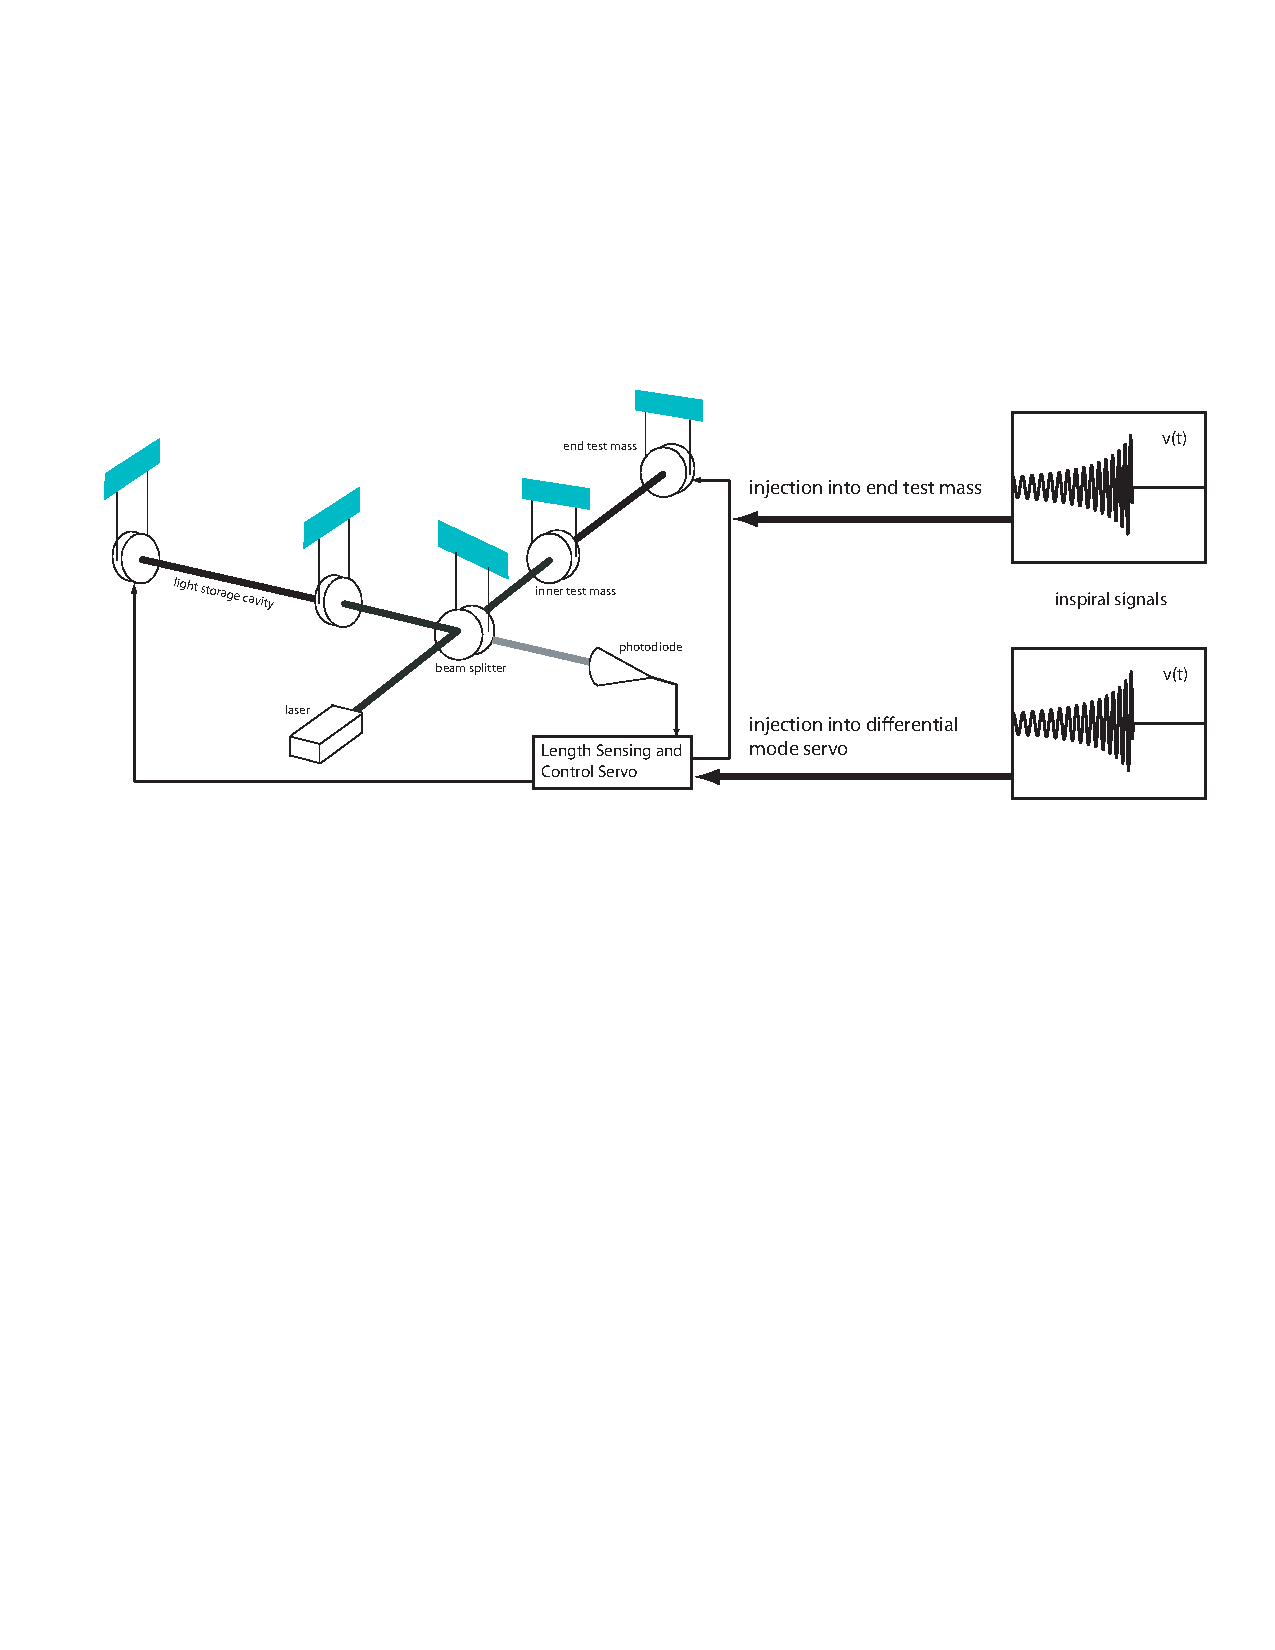
\includegraphics[width=\textwidth]{figures/hardware/ifo_inj}    
  \end{flushright}
  \caption[Schematic of LIGO Interferometer Showing Injection Points]{%
  A schematic diagram of the LIGO interferometer showing the injection points
  used in S1 hardware injections. Inspiral signals were injected either
  directly into the end test mass drive of one arm or into the differential
  mode servo, and this into both arms. Care was taken to ensure that the
  correct transfer function, $T(f)$, was used in each case.
  }
\label{f:ifo_inj}
\end{figure}

\begin{figure}[p]
  \vspace{5pt}
  \begin{flushright}
    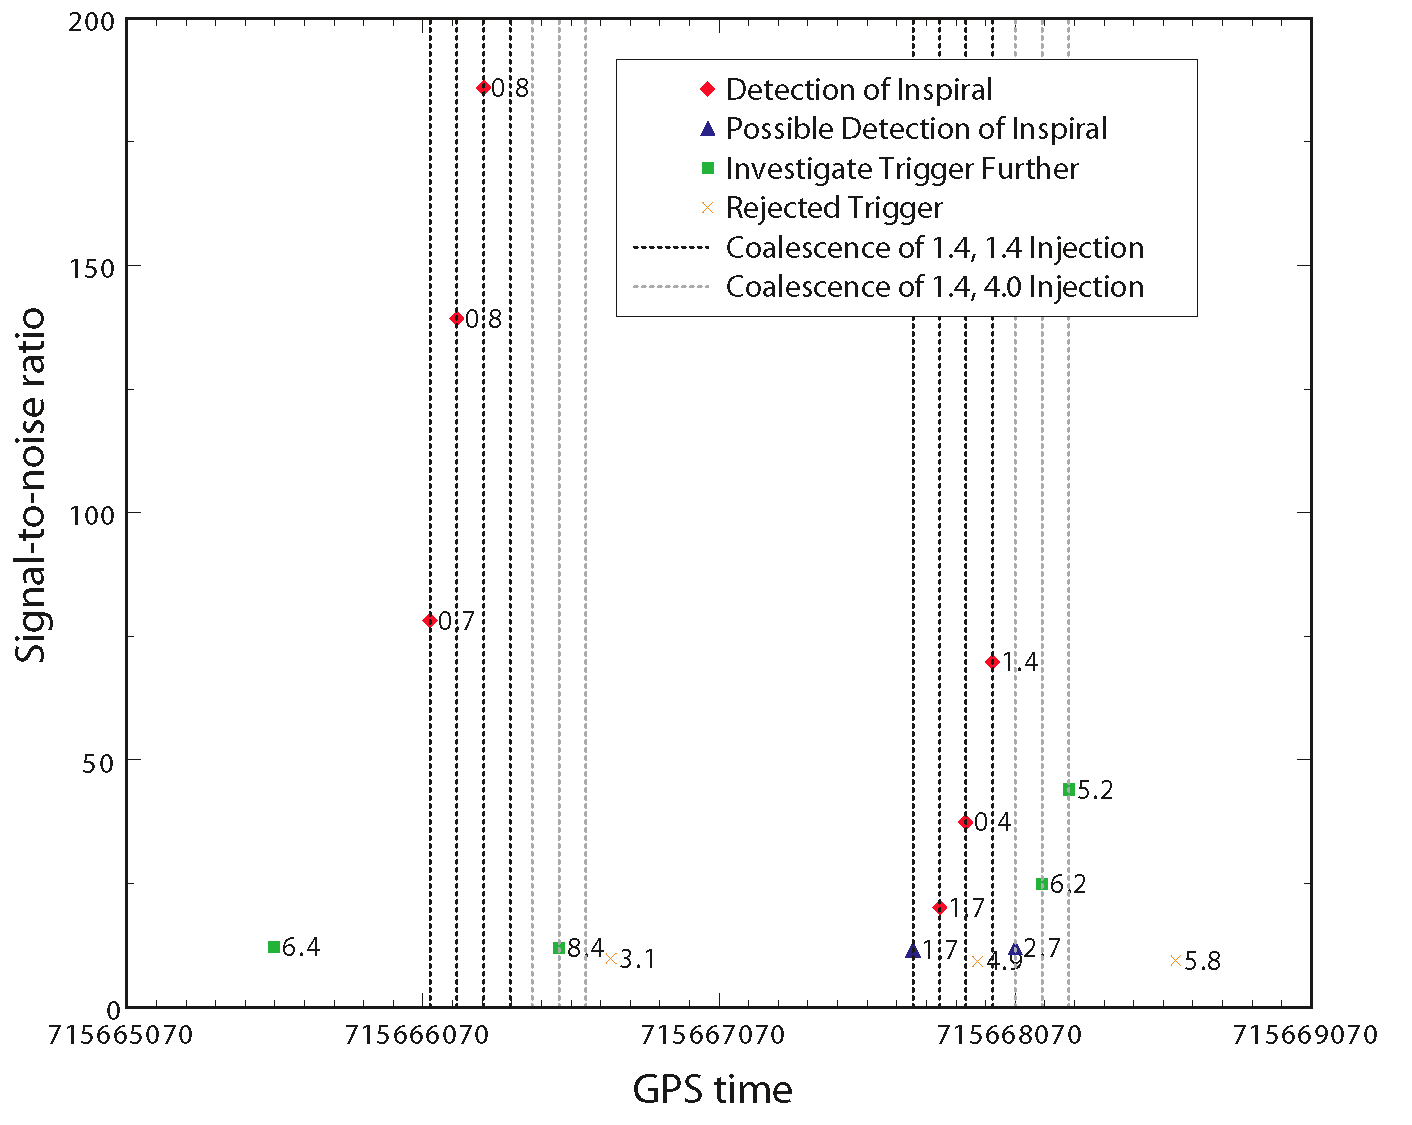
\includegraphics[width=\textwidth]{figures/hardware/inj_snr}    
  \end{flushright}
  \caption[Candidate Events from Hardware Injections]{%
The candidate events generated by processing 4000 seconds of data from the
Livingston 4 km interferometer through the S1 analysis pipeline.  This data
included two sets of injections; the known coalescence times are indicated by
the dashed vertical lines. The signal-to-noise ratio is plotted and the value
of the $\chi^2$ veto is shown next to the candidate event.
  }
\label{f:inj_snr}
\end{figure}

\begin{table}[p]
  \begin{flushright}
  \begin{tabular}{l|l|c|c}
  End time of Injection&End Time of Detection&$\rho$&$\chi^2$\\
  \hline
  $04:35:12.424928$ & $04:35:12.424927$ & $11.623546$ & $1.653222$ \\
  $04:36:42.424928$ & $04:36:42.425171$ & $20.230101$ & $1.671016$ \\
  $04:38:12.424928$ & $04:38:12.424927$ & $37.488770$ & $0.443966$ \\
  $04:39:42.424928$ & $04:39:42.424927$ & $69.815262$ & $1.375486$ \\
  \end{tabular}
  \end{flushright}
  \caption[Hardware Injections Found by the Analysis Pipeline]{%
  Hardware injection events found by the inspiral analysis pipeline. End time
  of injection is the known end time of the injected signal and end time of
  detection is the end time of the signal as reported by the analysis
  pipeline. Times are Universal Time (UTC) on 10 September 2002. The values of
  signal-to-noise ratio $\rho$ and $\chi^2$ veto are given for each event.
  }
\label{t:triggers}
\end{table}

\begin{figure}[p]
  \vspace{5pt}
  \begin{flushright}
    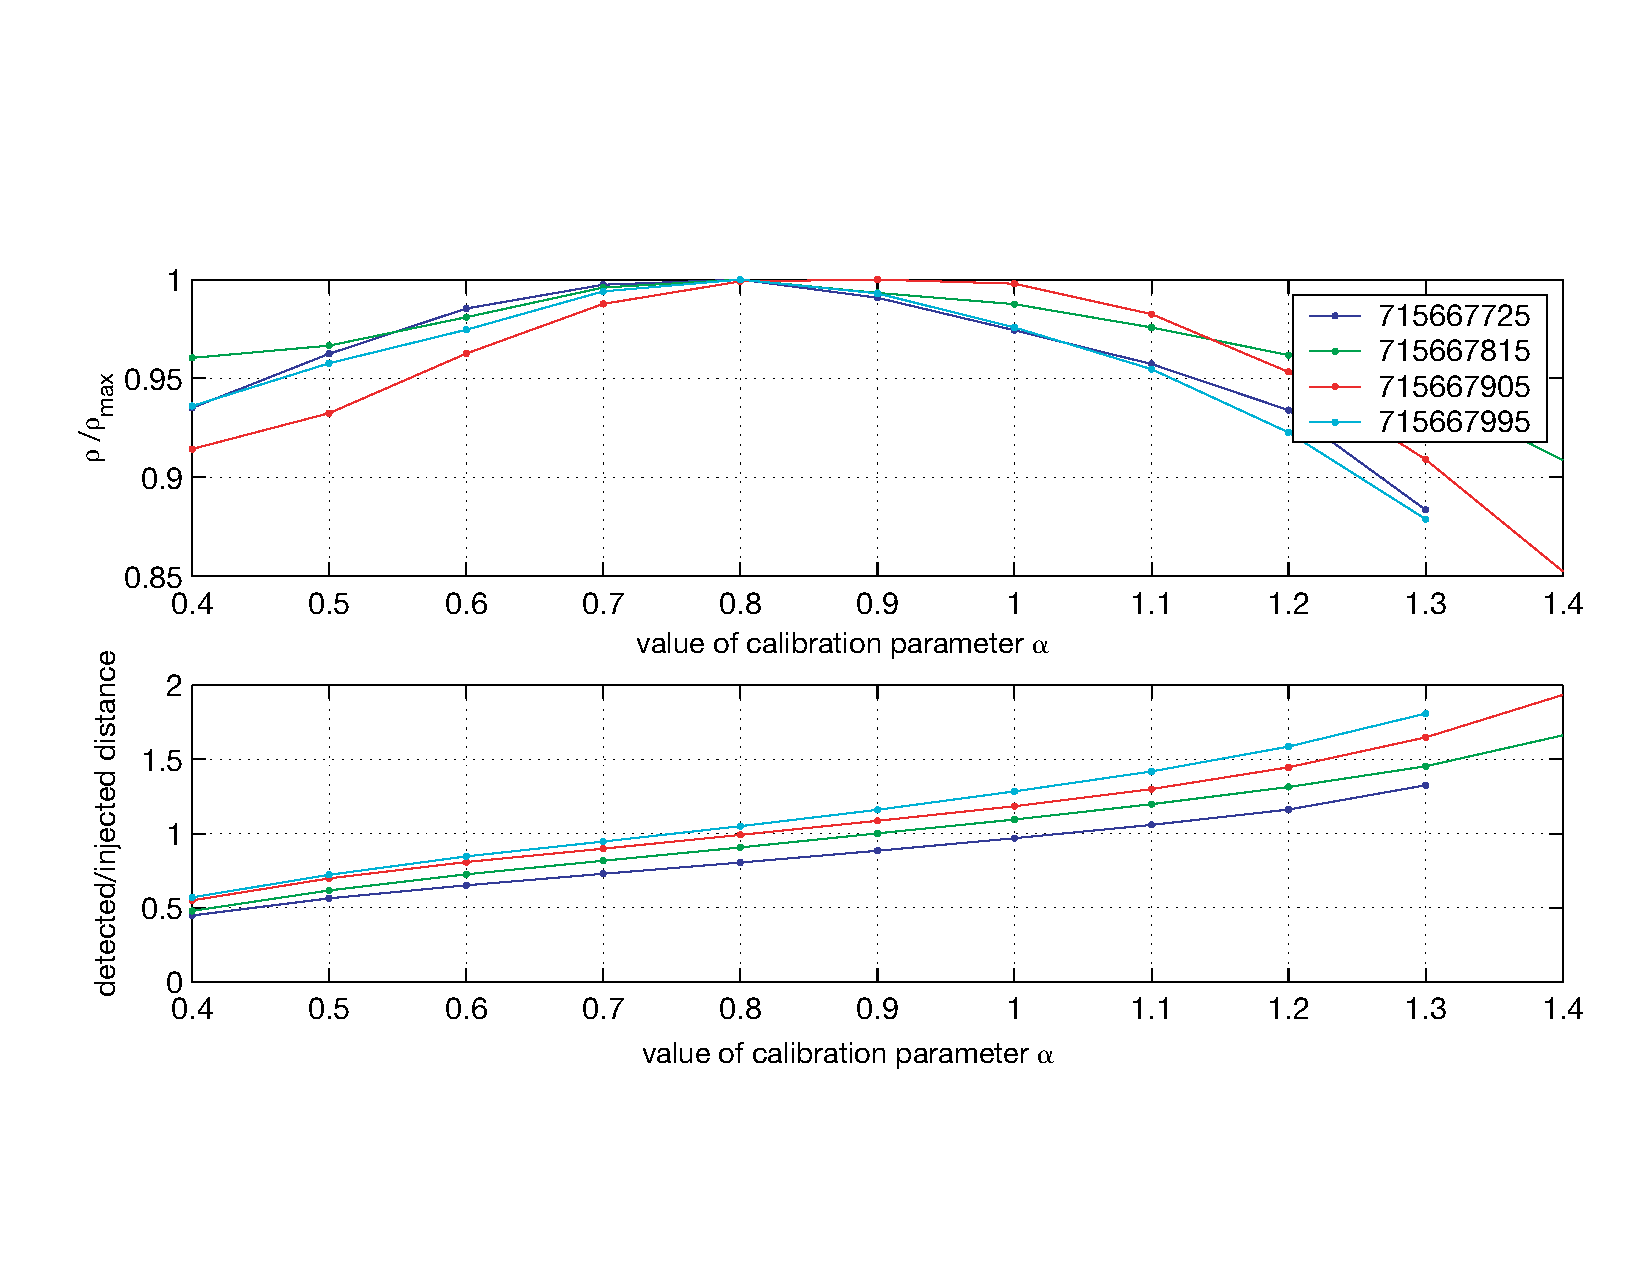
\includegraphics[width=\textwidth]{figures/hardware/calibration}    
  \end{flushright}
  \caption[Study of Calibration Using Hardware Injections]{%
  Each curve corresponds to a hardware injection at the given GPS time. We
  re-analyze each injection with different calibrations to show how the
  detected quantities vary with $\alpha$. The upper plot shows the ratio of
  signal-to-noise ratio, $\rho$, to its maximum value, $\rho_{\mathrm{max}}$.
  The lower plot shows ratio of the detected distance to the known distance of
  the hardware injection.
  }
\label{f:calibration}
\end{figure}

\begin{figure}[p]
  \vspace{5pt}
  \begin{flushright}
    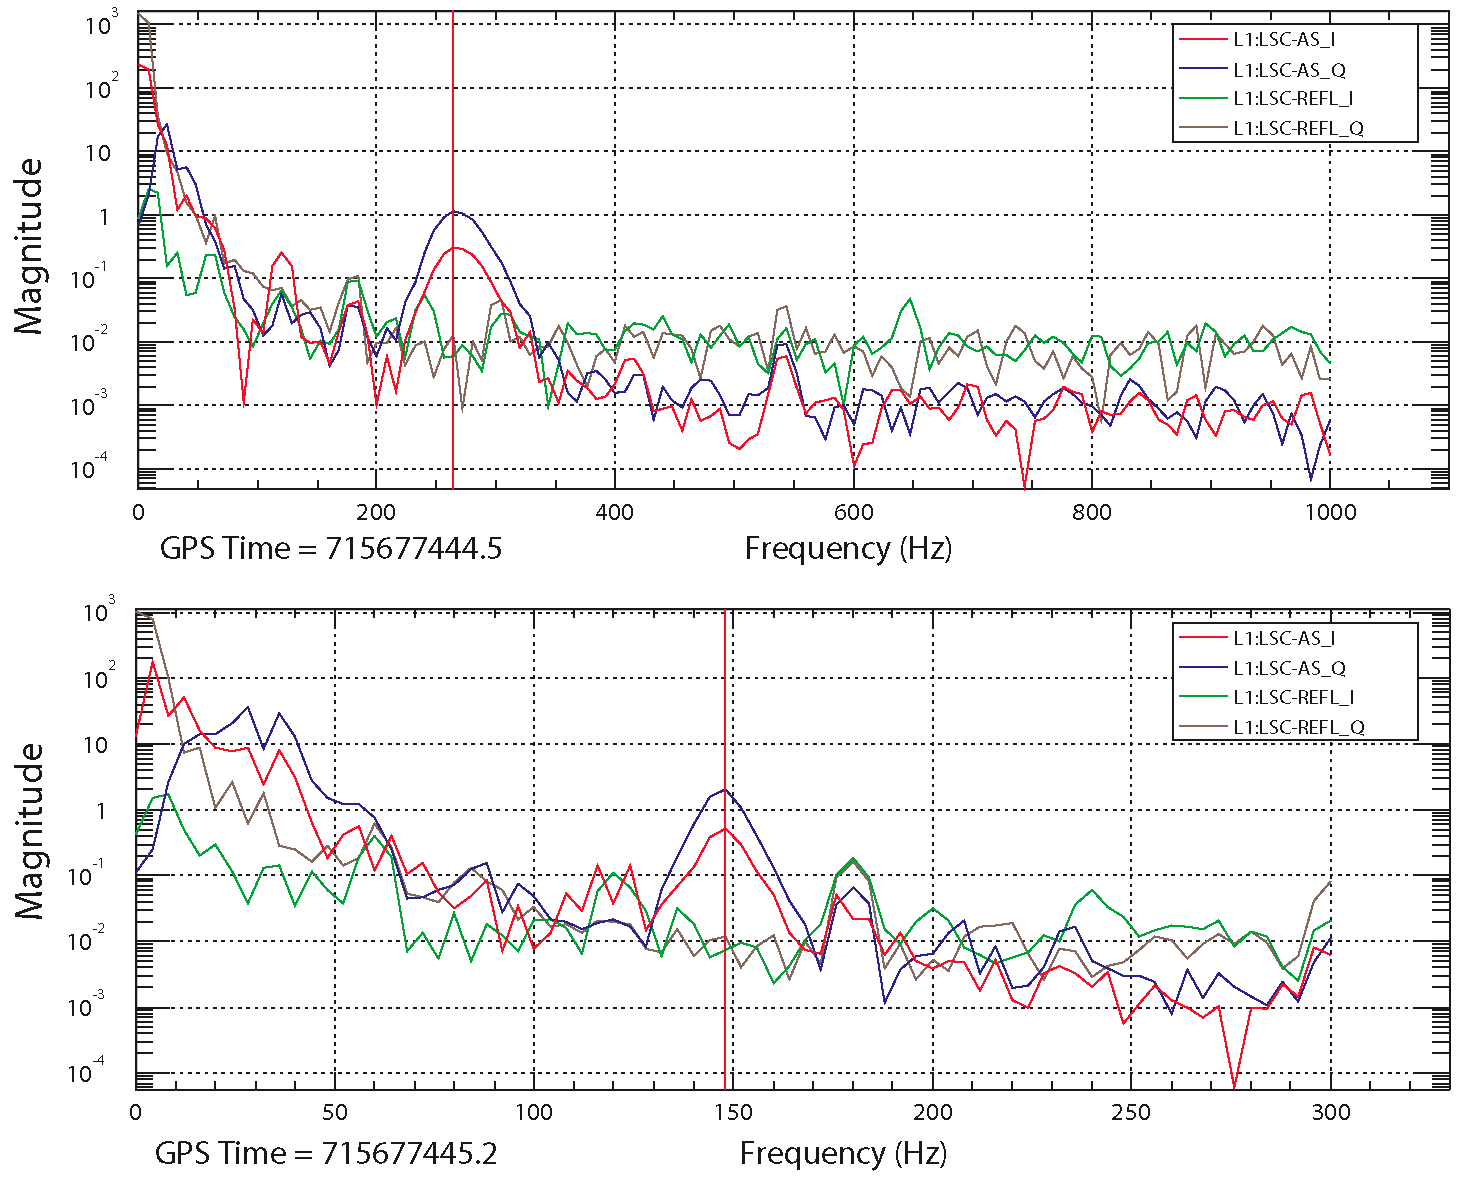
\includegraphics[width=\textwidth]{figures/hardware/veto_safe}    
  \end{flushright}
  \caption[Study of Veto Safety Using Hardware Injections]{%
  Power spectra of the gravitational wave channel LSC-AS\_Q and the auxiliary
  channels LSC-AS\_I, LSC-REFL\_I and LSC-REFL\_Q during a 
  hardware injection. The broad peak in the spectrum is the inspiral signal
  and the two power spectra taken at subsequent times show it sweeping across
  the band as the frequency of the inspiral signal increases with time.
  }
\label{f:veto_safe}
\end{figure}




